 \documentclass{article}
\usepackage{graphicx} % Required for inserting images
% header

%% natbib
\usepackage{natbib}
\bibliographystyle{plain}

%% comment
\usepackage{comment}

% no automatic indentation
\usepackage{indentfirst}

% manually indent
\usepackage{xargs} % \newcommandx
\usepackage{calc} % calculation
\newcommandx{\tab}[1][1=1]{\hspace{\fpeval{#1 * 10}pt}}
% \newcommand[number of parameters]{output}
% \newcommandx[number of parameters][parameter index = x]{output}
% use parameter index = x to substitute the default argument
% use #1, #2, ... to get the first, second, ... arguments
% \tab for indentation
% \tab{2} for for indentation twice

% note
\newcommandx{\note}[1]{\textit{\textcolor{red}{#1}}}
\newcommand{\todo}{\note{TODO}}
% \note{TODO}

%% math package
\usepackage{amsfonts}
\usepackage{amsmath}
\usepackage{amssymb}
\usepackage{tikz-cd}
\usepackage{mathtools}
\usepackage{amsthm}

%% operator
\DeclareMathOperator{\tr}{tr}
\DeclareMathOperator{\diag}{diag}
\DeclareMathOperator{\sign}{sign}
\DeclareMathOperator{\grad}{grad}
\DeclareMathOperator{\curl}{curl}
\DeclareMathOperator{\Div}{div}
\DeclareMathOperator{\card}{card}
\DeclareMathOperator{\Span}{span}
\DeclareMathOperator{\real}{Re}
\DeclareMathOperator{\imag}{Im}
\DeclareMathOperator{\supp}{supp}
\DeclareMathOperator{\im}{im}
\DeclareMathOperator{\aut}{Aut}
\DeclareMathOperator{\inn}{Inn}
\DeclareMathOperator{\Char}{char}
\DeclareMathOperator{\Sylow}{Syl}
\DeclareMathOperator{\coker}{coker}
\DeclareMathOperator{\inc}{in}
\DeclareMathOperator{\Sd}{Sd}
\DeclareMathOperator{\Hom}{Hom}
\DeclareMathOperator{\interior}{int}
\DeclareMathOperator{\ob}{ob}
\DeclareMathOperator{\Set}{Set}
\DeclareMathOperator{\Top}{Top}
\DeclareMathOperator{\Meas}{Meas}
\DeclareMathOperator{\Grp}{Grp}
\DeclareMathOperator{\Ab}{Ab}
\DeclareMathOperator{\Ch}{Ch}
\DeclareMathOperator{\Fun}{Fun}
\DeclareMathOperator{\Gr}{Gr}
\DeclareMathOperator{\End}{End}
\DeclareMathOperator{\Ad}{Ad}
\DeclareMathOperator{\ad}{ad}
\DeclareMathOperator{\Bil}{Bil}
\DeclareMathOperator{\Skew}{Skew}
\DeclareMathOperator{\Tor}{Tor}
\DeclareMathOperator{\Ho}{Ho}
\DeclareMathOperator{\RMod}{R-Mod}
\DeclareMathOperator{\Ev}{Ev}
\DeclareMathOperator{\Nat}{Nat}
\DeclareMathOperator{\id}{id}
\DeclareMathOperator{\Var}{Var}
\DeclareMathOperator{\Cov}{Cov}
\DeclareMathOperator{\RV}{RV}
\DeclareMathOperator{\rank}{rank}

%% pair delimiter
\DeclarePairedDelimiter{\abs}{\lvert}{\rvert}
\DeclarePairedDelimiter{\inner}{\langle}{\rangle}
\DeclarePairedDelimiter{\tuple}{(}{)}
\DeclarePairedDelimiter{\bracket}{[}{]}
\DeclarePairedDelimiter{\set}{\{}{\}}
\DeclarePairedDelimiter{\norm}{\lVert}{\rVert}

%% theorems
\newtheorem{axiom}{Axiom}
\newtheorem{definition}{Definition}
\newtheorem{theorem}{Theorem}
\newtheorem{proposition}{Proposition}
\newtheorem{corollary}{Corollary}
\newtheorem{lemma}{Lemma}
\newtheorem{remark}{Remark}
\newtheorem{claim}{Claim}
\newtheorem{problem}{Problem}
\newtheorem{assumption}{Assumption}
\newtheorem{example}{Example}
\newtheorem{exercise}{Exercise}

%% empty set
\let\oldemptyset\emptyset
\let\emptyset\varnothing

\newcommand\eps{\epsilon}

% mathcal symbols
\newcommand\Tau{\mathcal{T}}
\newcommand\Ball{\mathcal{B}}
\newcommand\Sphere{\mathcal{S}}
\newcommand\bigO{\mathcal{O}}
\newcommand\Power{\mathcal{P}}
\newcommand\Str{\mathcal{S}}


% mathbb symbols
\usepackage{mathrsfs}
\newcommand\N{\mathbb{N}}
\newcommand\Z{\mathbb{Z}}
\newcommand\Q{\mathbb{Q}}
\newcommand\R{\mathbb{R}}
\newcommand\C{\mathbb{C}}
\newcommand\F{\mathbb{F}}
\newcommand\T{\mathbb{T}}
\newcommand\Exp{\mathbb{E}}

% mathrsfs symbols
\newcommand\Borel{\mathscr{B}}

% algorithm
\usepackage{algorithm}
\usepackage{algpseudocode}

% longproof
\newenvironment{longproof}[1][\proofname]{%
  \begin{proof}[#1]$ $\par\nobreak\ignorespaces
}{%
  \end{proof}
}


% for (i) enumerate
% \begin{enumerate}[label=(\roman*)]
%   \item First item
%   \item Second item
%   \item Third item
% \end{enumerate}
\usepackage{enumitem}

% insert url by \url{}
\usepackage{hyperref}

% margin
\usepackage{geometry}
\geometry{
a4paper,
total={190mm,257mm},
left=10mm,
top=20mm,
}


\title{ma5209 assignment 1}
\author{Nguyen Ngoc Khanh - A0275047B}
\date{February 2024}

\begin{document}

\maketitle

\begin{problem}
    Let $\Omega$ be an open subset of $\R^2$. Write $\mathscr{C}^\infty(\Omega)$ for the vector space of smooth ($C^\infty$) functions on $\Omega$ and $\mathscr{VF}^\infty(\Omega)$ for the vector space of smooth ($C^\infty$) vector fields on $\Omega$. Recall the operators
\begin{center}
% https://tikzcd.yichuanshen.de/#N4Igdg9gJgpgziAXAbVABwnAlgFyxMJZABgBpiBdUkANwEMAbAVxiRAB12BbOnACzgBjAE7AAwgF8AepyxgAZjgCeACk4B5LjADmdAJQgJpdJlz5CKAIzkqtRizace-IaIBqAMWmyFyte00dfUNjEAxsPAIiACYbanpmVkQObl4BEXFvdjlFVQ0tXQMJWxgobXgiUHlhCC4kMhAcCCRrO0THdm1hOigQqpq6xFampFi2h2TOQSZhBkMKCSA
\begin{tikzcd}
\mathscr{C}^\infty(\Omega) \arrow[r, "\grad"] & \mathscr{VF}^\infty(\Omega) \arrow[r, "\curl"] & \mathscr{C}^\infty(\Omega)
\end{tikzcd}
\end{center}
    the relation
    $$
        \curl \circ \grad = 0
    $$
    and the notation
    $$
        H^0_{dR} = \ker(\grad), \; H^1_{dR} = \frac{\ker(\curl)}{\im(\grad)}, \; H^2_{dR} = \coker(\curl)
    $$
    For \ref{1.1}-\ref{1.3} suppose $\Omega = \R^2 - \set{p, q}$ where $p, q$ are distinct points of $\R^2$. Let $\sigma_1: \Delta^1 \to \Omega$ be defined (in terms of the barycentric coordinates $(x_0, x_1)$ on $\Delta^1$) by $\sigma_1(x_1) = p + \frac{\norm{p-q}}{3} \begin{bmatrix} \cos(2\pi x_1) \\ \sin(2\pi x_1)\end{bmatrix}$ and $\sigma_2: \Delta^1 \to \Omega$ by $\sigma_2(x_1) = q + \frac{\norm{p-q}}{3} \begin{bmatrix} \cos(2\pi x_1) \\ \sin(2\pi x_1)\end{bmatrix}$. Define $\sigma: \Delta^1 \to \Omega$ by $\sigma(x_1) = \frac{p+q}{2} + \norm{p-q} \begin{bmatrix} \cos(2\pi x_1) \\ \sin(2\pi x_1)\end{bmatrix}$

    \begin{enumerate}[label=(\roman*)]
        \item \label{1.1} Verify that $\sigma_1, \sigma_2$ and $\sigma$ are singular $1$-cycles. Then establish a linear relation between their classes in the singular homology $H_1(\Omega)$. A picture is worth a thousand words.
        \item \label{1.2} Represent the homology class $2[\sigma_1]$ by a single $1$-cycle. To do this you must write down the $1$-cycle and a homology between it and $2\sigma_1$
        \item \label{1.3} Let us grant that $H_1(\Omega)$ is generated by the classes of $\sigma_1$ and $\sigma_2$. Construct a surjective homomorphism $H^1_{dR}(\Omega) \to \Hom(H_1(\Omega), \R)$
        \item \label{1.4} For some reasonable class of open subsets of $\R^2$, construct a bijective homomorphism $H^1_{dR}(\Omega) \to \Hom(H_1(\Omega), \R)$
        \item \label{1.5} Say something sensible about $H^2_{dR}(\Omega)$ for some class of open subsets $\Omega$ of $\R^2$
    \end{enumerate}
\end{problem}

\begin{longproof}
    \ref{1.1}
    
    Some geometric observations:
    \begin{itemize}
        \item The image of $\sigma_1$ is a circle of radius $\frac{\norm{p-q}}{3}$ centers at $p$, encloses only $p$ with $\sigma_1(0) = \sigma_1(1)$
        \item The image of $\sigma_2$ is a circle of radius $\frac{\norm{p-q}}{3}$ centers at $q$, encloses only $q$ with $\sigma_2(0) = \sigma_2(1)$
        \item The image of $\sigma$ is a circle of radius $\norm{p-q}$ centers at $\frac{p+q}{2}$, encloses $p$, $q$, $\sigma_1, \sigma_2$ with $\sigma(0) = \sigma(1)$
    \end{itemize}

    As $\sigma \in S_1(\Omega)$, let $\partial: C_1(\Omega) \to C_0(\Omega)$ be the boundary operator at dimension $1$, then $\partial \sigma \in C_0(\Omega)$ is
    \begin{align*}
        \partial \sigma
        &= \sum_{i=0}^1 (-1)^i \sigma d^i \\
        &= \sigma \circ d^0 - \sigma \circ d^1
    \end{align*}
    where $d^0: \Delta^0 \to \Delta^1$ is an affine map that maps vertex $0$ of $\Delta^0$ to vertex $1$ of $\Delta^1$, $d^1: \Delta^0 \to \Delta^1$ is an affine map that maps vertex $0$ of $\Delta^0$ to vertex $0$ of $\Delta^1$. Then
    \begin{align*}
        \sigma \circ d^0 &= \Delta^0 \mapsto \sigma(1) \\
        \sigma \circ d^1 &= \Delta^0 \mapsto \sigma(0)
    \end{align*}
    As $\sigma(1) = \sigma(0)$, $\partial \sigma = 0$, $\sigma$ is a $1$-cycle. Similar treatments for $\sigma_1, \sigma_2$ show $\sigma_1, \sigma_2$ being $1$-cycles.

    \begin{figure}[h]
    \centering
    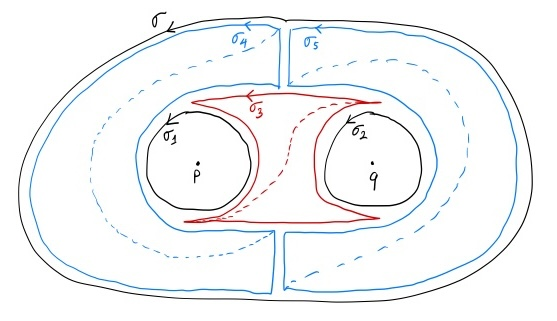
\includegraphics[width=0.5\textwidth]{1.1.jpg}
    \caption{A picture is worth a thousand words}
    \label{fig_1.1}
    \end{figure}

    Next we define $\sigma_3, \sigma_4, \sigma_5 \in C_1(\Omega)$ as shown in figure \ref{fig_1.1} (each is a sum of 4 singular $1$-simplices). As $\sigma_3, \sigma_4, \sigma_5$ are boundaries (by the triangularization), then $[\sigma] = [\sigma_1 + \sigma_2] = [\sigma_1] + [\sigma_2]$

    \ref{1.2}
    
    Let $\sigma_3: \Delta^1 \to \Omega$ be defined by $\sigma_3(x_1) = p + \frac{\norm{p-q}}{3} \begin{bmatrix} \cos(4\pi x_1) \\ \sin(4\pi x_1)\end{bmatrix}$ (this cycle wraps around $p$ twice). Then, consider the singular $2$-simplex $\sigma$ such that $d_0 \sigma = d_2 \sigma = \sigma_1$ and $d_1 \sigma = \sigma_3$ as in figure \ref{fig_1.2}
    
    \begin{figure}[h]
    \centering
    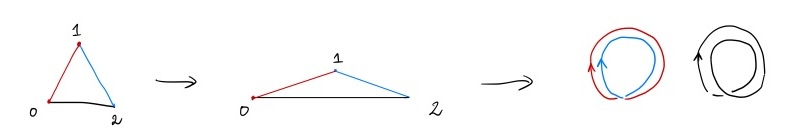
\includegraphics[width=0.5\textwidth]{1.2.jpg}
    \caption{A picture is worth a thousand words}
    \label{fig_1.2}
    \end{figure}

    The boundary of $\sigma$ is
    \begin{align*}
        \partial \sigma
        &= d_0 \sigma - d_1 \sigma + d_2 \sigma \\
        &= \sigma_1 - \sigma_3 + \sigma_1
    \end{align*}

    Then $0 = [\partial \sigma] = 2 [\sigma_1] - [\sigma_3]$. That is, $[\sigma_3] = 2[\sigma_1]$

    \ref{1.3}
    
    $H_1(\Omega) = \inner{[\sigma_1], [\sigma_2]} = \Z \oplus \Z$ is a free abelian group generated by $\set{[\sigma_1], [\sigma_2]}$. Let $f \in \Hom(H_1(\Omega), \R)$, let $p = f([\sigma_1]) \in \R, q = f([\sigma_2]) \in \R$. Then, for any element $a [\sigma_1] + b[\sigma_2] \in H_1(\Omega)$, as $f$ is a homomorphism,
    $$
        f (a[\sigma_1] + b[\sigma_2]) = ap + bq
    $$
    The pair $(p, q) \in \R \oplus \R$ determines $f$, that is, $\Hom(H_1(\Omega), \R) = \R \oplus \R$.

    Now, let $V \in \ker(\curl)$, and let
    \begin{align*}
        p(V) &= \oint_{\sigma_1} \overrightarrow{V} \cdot d\overrightarrow{r} \in \R\\
        q(V) &= \oint_{\sigma_2} \overrightarrow{V} \cdot d\overrightarrow{r} \in \R
    \end{align*}

    Let $\phi: \ker(\curl) \to \R \oplus \R$ be defined by
    $$
        \phi(V) = (p(V), q(V))
    $$

\begin{center}
% https://tikzcd.yichuanshen.de/#N4Igdg9gJgpgziAXAbVABwnAlgFyxMJZABgBpiBdUkANwEMAbAVxiRAB12BrGAJwApOAYya8GAShABfUuky58hFGQCMVWoxZsAEgD0V4gPrAovKYPYB5ALYwA5nXEACALxPOAM150hwTjwFhUQkpP3Ysaws7byhxKWlZEAxsPAIiACZydXpmVkQOdm0ISO1DFQsbe0dSd3YAJUkpdRgoO3giUC9ipDIQHAgkTI1ctk40AAssBM7ebsQVan7B6hytfLHJ6ZAu6x7FgfnqcZg6KDYcAHcIY9OEJqkgA
\begin{tikzcd}
\ker(\curl) \arrow[rr, "\phi"] \arrow[d, two heads]                    &  & {\Hom(H_1(\Omega), \R) = \R \oplus \R} \\
H^1_{dR}(\Omega) = \frac{\ker(\curl)}{\im(\grad)} \arrow[rru, "\phi"] &  &                        
\end{tikzcd}
\end{center}

    We claim that the extension of $\phi$ to $H^1_{dR}(\Omega)$ is a surjective homomorphism. Firstly, we will verify that $\phi: H^1_{dR}(\Omega) \to \Hom(H_1(\Omega), \R)$ is well-defined. Let $[V_1] = [V_2] \in H^1_{dR}(\Omega)$, that is, $V_1, V_2$ in the same coset, then $V_2 = V_1 + B$ where $B \in \im(\grad)$, we have
    \begin{align*}
        p(V_2) &= \oint_{\sigma_1} \overrightarrow{V_2} \cdot d\overrightarrow{r} = \oint_{\sigma_1} (\overrightarrow{V_1} + \overrightarrow{B}) \cdot d\overrightarrow{r} = \oint_{\sigma_1} \overrightarrow{V_1} \cdot d\overrightarrow{r} + \oint_{\sigma_1} \overrightarrow{B} \cdot d\overrightarrow{r} = \oint_{\sigma_1} \overrightarrow{V_1} \cdot d\overrightarrow{r} = p(V_1) \\
        q(V_2) &= \oint_{\sigma_2} \overrightarrow{V_2} \cdot d\overrightarrow{r} = \oint_{\sigma_2} (\overrightarrow{V_1} + \overrightarrow{B}) \cdot d\overrightarrow{r} = \oint_{\sigma_2} \overrightarrow{V_1} \cdot d\overrightarrow{r} + \oint_{\sigma_2} \overrightarrow{B} \cdot d\overrightarrow{r} = \oint_{\sigma_2} \overrightarrow{V_1} \cdot d\overrightarrow{r} = q(V_1)
    \end{align*}
    Secondly, $\phi([V_1] + [V_2]) = \phi[V_1] + \phi[V_2]$ for all $[V_1], [V_2] \in H^1_{dR}(\Omega)$ (the addition in RHS is element-wise addition in $\R \oplus \R$)
    \begin{align*}
        \phi([V_1] + [V_2])
        &= \phi([V_1 + V_2]) \\
        &= \tuple*{\oint_{\sigma_1} (\overrightarrow{V_1} + \overrightarrow{V_2}) \cdot d\overrightarrow{r}, \oint_{\sigma_2} (\overrightarrow{V_1} + \overrightarrow{V_2}) \cdot d\overrightarrow{r} } \\
        &= \tuple*{\oint_{\sigma_1} \overrightarrow{V_1} \cdot d\overrightarrow{r} + \oint_{\sigma_1} \overrightarrow{V_2} \cdot d\overrightarrow{r}, \oint_{\sigma_2} \overrightarrow{V_1} \cdot d\overrightarrow{r} + \oint_{\sigma_2} \overrightarrow{V_2} \cdot d\overrightarrow{r} } \\
        &= \tuple*{\oint_{\sigma_1} \overrightarrow{V_1} \cdot d\overrightarrow{r}, \oint_{\sigma_2} \overrightarrow{V_1} \cdot d\overrightarrow{r}} + \tuple*{\oint_{\sigma_1} \overrightarrow{V_2} \cdot d\overrightarrow{r}, \oint_{\sigma_2} \overrightarrow{V_2} \cdot d\overrightarrow{r} } \\
        &= \phi[V_1] + \phi[V_2]
    \end{align*}
    Thirdly, $\phi$ is surjective. Because there exists vector fields $V_1, V_2 \in \ker(\curl)$ such that $\phi[V_1] = (1, 0)$ and $\phi[V_2] = (0, 1)$. Then for any pair $(p, q) \in \R \oplus \R$, the vector field $V = p V_1 + q V_2$ will have $\phi(V) = (p, q)$

    \ref{1.4}

    For any simply connected subset $\Omega$ of $\R^2$, by Green theorem, $\im (\grad) = \ker(\curl)$. Both $H^1_{dR}(\Omega)$ and $\Hom(H_1(\Omega), \R)$ are trivial groups. The homomorphism in \ref{1.3} is bijective.

    For any simply connected subset $\Omega$ of $\R^2$ with one missing point $p$. There is a homotopy equivalence between $\Omega$ and $S^1$, hence $H_1(\Omega) = H_1(S^1) = \Z$ and $H_1(\Omega)$ is generated by a circle containing in its interior, namely $\sigma$. The homomorphism in \ref{1.3} is surjective. The injectivity follows from if $V \in \ker \phi$, then $V \in \im \grad$. That is, if $\oint_\sigma \overrightarrow{V} \cdot d\overrightarrow{r} = 0$, then $V \in \im \grad$. This can be done if $\oint_\sigma \overrightarrow{V} \cdot d\overrightarrow{r} = 0$ implies that we can assign a value of $V$ at the missing point $p$ such that the new vector field is still smooth.

    \ref{1.5} 
    As $\curl$ is surjective,
    $$
        \coker(\curl) = \frac{\mathscr{C}^\infty(\Omega)}{\im(\curl)} = 1
    $$
\end{longproof}

\begin{problem}
    Verify the identities $d^j \circ d^i = d^i \circ d^{j-1}$ and $d_i d_j = d_{j-1} d_i$ if $i < j$. Use this identity to verify the identity $\partial^2 = 0$ in the singular chain complex of a space.
\end{problem}

\begin{longproof}
    Let $[v_0, v_1, ..., v_n]$ a sequence of $n+1$ symbols where each symbol is from $\set{0, 1, ..., m} + \set{*}, m \leq n$ denote the affine map $\Delta^m \to \Delta^n$ such that the $i$th vertex of $\Delta^n$ is mapped from $v_i$th vertex of $\Delta^m$. For example, $[0, 2, *, 1]$ denotes the affine map $\Delta^2 \to \Delta^3$ such that $0 \mapsto 0$, $2 \mapsto 1$, $1 \mapsto 3$. Then a face map $d^i$ for $i \leq n+1$ inserts the $*$ symbol to the $i$th position
    $$
        d^i: [v_0, v_1, ..., v_n] \mapsto [v_0, v_1, v_{i-1}, *, v_i, ..., v_n]
    $$

    Let $e = [0, 1, ..., n-1]: \Delta^{n-1} \to \Delta^{n-1}$ be the identity map. Then
    \begin{align*}
        \Delta^{n-1} \to \Delta^n: d^i(e) &= [0, 1, .., i-1, *_1, i, ..., n-1] \\
        \Delta^{n-1} \to \Delta^{n+1}: (d^j \circ d^i)(e) &= \begin{cases}
            [0, 1, ..., i-1 = j-2, *_1, *_2, i = j-1, ..., n-1], & i = j-1 \\
            [0, 1, ..., i-1, *_1, i, ..., j-2, *_2, j-1, ..., n-1], & i < j-1
        \end{cases} \\
        \Delta^{n-1} \to \Delta^n: d^{j-1}(e) &= [0, 1, .., j-2, *_1, j-1, ..., n-1] \\
        \Delta^{n-1} \to \Delta^{n+1}: (d^i \circ d^{j-1})(e) &= \begin{cases}
            [0, 1, ..., i-1 = j-2, *_2, *_1, i = j-1, ..., n-1], & i = j-1 \\
            [0, 1, ..., i-1, *_2, i, ..., j-2, *_1, j-1, ..., n-1], & i < j-1
        \end{cases} \\
    \end{align*}
    where $*_1, *_2$ are $*$ symbols, the subscripts are used to track the order. Hence, $d^j \circ d^i = d^i \circ d^{j-1}$, $d_i d_j = d_{j-1} d_i$ is immediate. Now, we will verify $\partial^2 = 0$. Let $\sigma \in C_n(X)$, then
    \begin{align*}
        \partial^2 \sigma
        &= \sum_{j=0}^{n-1} (-1)^j \tuple*{\sum_{i=0}^n (-1)^i \sigma \circ d^i} \circ d^j \\
        &= \sum_{j=0}^{n-1} \sum_{i=0}^n (-1)^j (-1)^i \sigma \circ d^i \circ d^j
    \end{align*}
    Split the set of $(i, j)$ indices into two subsets of the same size $A = \set{i > j}, B = \set{i \leq j}$ (each subset is of $n(n+1)/2$ elements). We define a bijection between $A$ and $B$ as follows: for each pair $(i_1, j_1) \in A$, let $(i_2, j_2) \in B$ be defined as $(i_2 = j_1+1, j_2 = i_1)$. We also observe that $(-1)^{j_1} (-1)^{i_1} + (-1)^{j_2} (-1)^{i_2} = 0$. Then, summing over the $n(n+1)/2$ pairs
    \begin{align*}
        \partial^2 \sigma 
        &= \sum_{(i_1, j_1), (i_2, j_2)} (-1)^{j_1} (-1)^{i_1} \sigma \circ d^{i_1} \circ d^{j_1} + (-1)^{j_2} (-1)^{i_2} \sigma \circ d^{i_2} \circ d^{j_2} \\
        &= \sum_{(i_1, j_1), (i_2, j_2)} (-1)^{j_1} (-1)^{i_1} \sigma \circ d^{i_1} \circ d^{j_1} + (-1)^{j_2} (-1)^{i_2} \sigma \circ d^{j_2} \circ d^{i_2-1} &\text{($d^{i_2} \circ d^{j_2} = d^{j_2} \circ d^{i_2-1}$)} \\
        &= \sum_{(i_1, j_1), (i_2, j_2)} (-1)^{j_1} (-1)^{i_1} \sigma \circ d^{i_1} \circ d^{j_1} + (-1)^{j_2} (-1)^{i_2} \sigma \circ d^{i_1} \circ d^{j_1} &\text{(by definition of the pairs)} \\
        &= \sum_{(i_1, j_1), (i_2, j_2)} [(-1)^{j_1} (-1)^{i_1} + (-1)^{j_2} (-1)^{i_2}] \sigma \circ d^{i_1} \circ d^{j_1} \\
        &= 0
    \end{align*}
\end{longproof}

\begin{problem}
    The $n$-sphere is $S^n = \set{x \in \R: \norm{x}=1}$. The homology of $S^n$ can be computed by writing it as a union of $U = S^n - \set{[0, ..., 0, -1]^T}$ and $V = S^n - \set{[0, ..., 0, 1]^T}$. Use this cover and the Mayer-Vietoris sequence of write down a cycle representing a generator of $H_1(S^1)$. Find another cycle consisting of a single $1$-simplex which is homologous to the generator you came up with. Then use the Mayer-Vietoris sequence again to find a $2$-cycle which represents a generator for $H_2(S^2)$. Is there a homologous $2$-cycle consisting of just one simplex?
\end{problem}
\begin{longproof}
    
    ($S^1$)
    
    In $S^1$ let $N = [0, 1]^T, S = [0, -1]^T, E = [1, 0]^T, W = [-1, 0]^T$. Let $U = S^1 - \set{S}, V = S^1 - \set{N}$, and an open cover $\mathcal{U} = \set{U, V}$. As $U, V$ contractible, 
    
    $$
        H_n(U) = H_n(V) = H_n(*) = \begin{cases}
            \Z, &n=0 \\
            0, &n > 0
        \end{cases}
    $$
    
    As $U, V$ has one path component, $U \cap V$ has two path components,
    $$
        H_0(U) = H_0(V) = \Z
    $$
    $$
        H_0(U \cap V) = \Z \oplus \Z
    $$
    
    Mayer-Vietoris sequence
    \begin{center}
    % https://tikzcd.yichuanshen.de/#N4Igdg9gJgpgziAXAbVABwnAlgFyxMJZABgBpiBdUkANwEMAbAVxiRAEZEQBfU9TXPkIoAzOSq1GLNgAkA+uwAUAVQCUAAgA6miGmZx18pQDUNAXnXEtOvUwPEefEBmx4CRAKzjq9Zqy5GigDCCgB62gC2dDgAFgDGjMDK3IoAyqHsquaGCmkZqo78rkJEZOwSvtJcxFy8RYLuKOyk5T5S-iDyxCrWCWjqpuoW2gBa1rr61iOFzgJuwshirZJ+snLdauO2Bl2Kg8OaY9oTdlM8EjBQAObwRKAAZgBOEBFIzSA4EEgATG2rXGg5AAqEDUBh0ABGMAYAAU5iUuAwYPccDMni8ftRPkgACx-KogbRoOiPPCMUEgcFQ2HwxogR5YK4xVF1EDo16IPEfL6ILwrAlYYEUqnQuHFOlIlHnbhAA
    \begin{tikzcd}
    1: &                                                &  & H_1(U) \oplus H_1(V) = 0 \oplus 0 \arrow[rr, "p_*"] &  & H_1(C_1^\mathcal{U}(S^1)) = H_1(S^1) \arrow[lllld, "\partial"'] \\
    0: & H_0(U \cap V) = \Z \oplus \Z \arrow[rr, "i_*"] &  & H_0(U) \oplus H_0(V) = \Z \oplus \Z                 &  &                                                                
    \end{tikzcd}
    \end{center}

    First isomorphism theorem on the connecting homomorphism $\partial$
    $$
        \frac{H_1(S^1)}{\ker \partial} = \im \partial
    $$
    
    By exactness at $H_1(S^1)$
    $$
        \ker \partial = \im p_* = \set{0}
    $$
    
    By exactness at $H_0(U \cap V)$
    $$
        \ker i_* = \im \partial
    $$

    Then
    $$
        H_1(S^1) = \ker i_*
    $$

    We have, $i_* = \begin{bmatrix} 1 & 1 \\ -1 & -1\end{bmatrix}: (a, b) \mapsto (a + b, - a - b)$. Then, $H_1(S^1) = \im \partial = \ker i_* = \Span \set*{\begin{bmatrix} 1 \\ -1\end{bmatrix}}$. In $\Z \oplus Z$, the subgroup $\Span \set*{\begin{bmatrix} 1 \\ -1\end{bmatrix}}$ is generated by $\begin{bmatrix} 1 \\ -1\end{bmatrix}$. Then, a cycle generating $H_1(S^1)$ is mapped into $\begin{bmatrix} 1 \\ -1\end{bmatrix}$ by $\partial$

    Recall the definition of the connecting homomorphism $\partial: H_{n+1}(C) \to H_n(A)$
    
    \begin{definition}[$\partial: H_{n+1}(C) \to H_n(A)$]
    Definition of the connecting homomorphism $\partial: H_{n+1}(C) \to H_n(A)$
    \begin{center}
        \begin{tikzcd}
        n+1  &                                                          & b \arrow[r, "p", maps to] \arrow[d, "\partial", maps to]          & c \arrow[d, "\partial", maps to] \\
        n:   & a \arrow[r, "i", maps to] \arrow[d, "\partial", maps to] & \partial b \arrow[r, "p", maps to] \arrow[d, "\partial", maps to] & 0                                \\
        n-1: & \partial a \arrow[r, "i", maps to]                       & \partial^2 b = 0                                                  &                                 
        \end{tikzcd}
    \end{center}

    Given $[c] \in H_{n+1}(C)$, (1) take any representative $c \in Z_{n+1}(C)$. As $p: B_{n+1} \to C_{n+1}$ is surjective, (2) take any $b \in B_{n+1}$ such that $pb = c$. As $p \partial b = \partial pb = \partial c = 0$ and $\ker (p: B_n \to C_n) = \im (i: A_n \to B_n)$, take $a \in A_n$ such that $ia = \partial b$, this choice is unique as $i$ is injective. $i \partial a = \partial i a = \partial^2 b = 0$, as $i$ is an injective homomorphism, $\partial a = 0$, then $a \in Z_n(A)$. The construction is done by $[c] \mapsto [a]$
    \end{definition}
    
    The diagram below is part of the short exact sequence $0 \to C_\bullet(U \cap V) \to C_\bullet(U) \oplus C_\bullet(V) \to C^\mathcal{U}_\bullet(S^1)$ that we will do diagram chasing on
    
\begin{comment}
    \begin{center}
% https://tikzcd.yichuanshen.de/#N4Igdg9gJgpgziAXAbVABwnAlgFyxMJZABgBoAmAXVJADcBDAGwFcYkQBhAfWIAoBVAAQAdYQGN6aQQDUAlCAC+pdJlz5CKchWp0mrdtz79ZI4RDQs4gw7zmLlIDNjwEiAFlLEdDFm0ScAPVEAW3ocAAsJRmB+BS4ARl4AZQD4kwBeawTk1PklFWd1Ii0vGh99f25E41NzSyzEuwUdGCgAc3giUAAzACcIYKQyEBwIJHiyvT8QLC5RAGJ7Hv7BxABmGlHxyd92UTR6XrwmJZA+gaQNkbHELV1d-zQ54UXmhSA
\begin{tikzcd}
                                 &  & C_1(U) \oplus C_1(V) \arrow[dd, "\partial"] \arrow[rr, "p_\#"] &  & C^\mathcal{U}_1(S^1) = C_1(S^1) \\
                                 &  &                                                                &  &                                 \\
C_0(U \cap V) \arrow[rr, "i_\#"] &  & C_0(U) \oplus C_0(V)                                           &  &                                
\end{tikzcd}
    \end{center}
\end{comment}

    \begin{figure}[h]
    \centering
    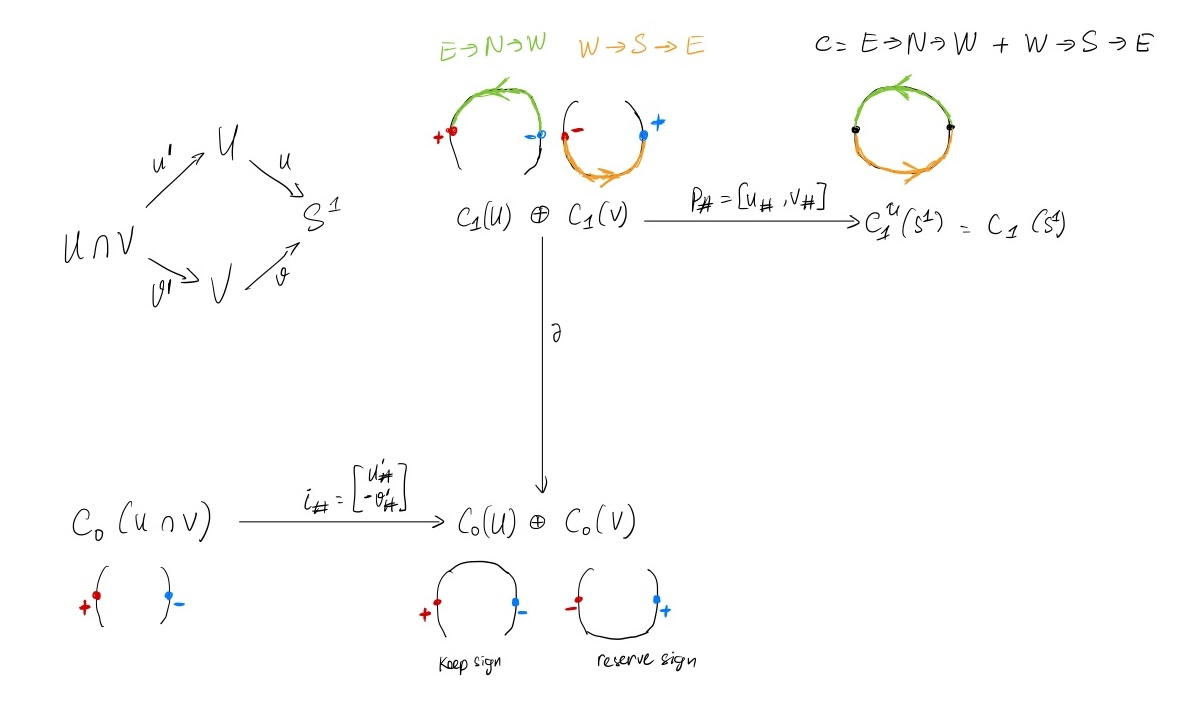
\includegraphics[width=0.7\textwidth]{3.1.jpg}
    \caption{A picture is worth a thousand words}
    \label{fig_3.1}
    \end{figure}

    Let $a = W - E \in C_0(U \cap V)$ be in the homology class of $\begin{bmatrix} 1 \\ -1\end{bmatrix} \in H_0(U \cap V)$, then $\partial b = (W - E, -W + E) \in C_0(U) \oplus C_0(V)$. Take $b = (E \to N \to W, W \to S \to E) \in C_1(U) \oplus C_1(V)$ where $x \to y \to z$ denotes the path (singular $1$-simplex) from $x$ to $y$ to $z$. Then $c = E \to N \to W + W \to S \to E$. $c$ is a cycle as $\partial c = W - E - W + E = 0$ and $[c]$ generates $H_1(S^1)$.

    Let $SE$ sits between $S$ and $E$. In the step of taking a pair of cycles having boundaries being $\partial b$, take $b_1 = (E \to SE \to E \to N \to W, W \to S \to E)$ and $\partial b_1 = \partial b$. Then $c_1 = E \to SE \to E \to N \to W + W \to S \to E$ and $[c_1] = [c]$

    The cycle $c_2 = E \to S \to W + W \to N \to E$ can be constructed in the similar fashion beginning with $a = -W + E$ that is in the homology class of $\begin{bmatrix} -1 \\ 1\end{bmatrix}$. And $[c_2] = -[c]$ also generates $H_1(S^1)$


    ($S^2$)

    In $S^2$, let $N = [0, 0, 1]^T, S = [0, 0, -1]^T$. Let $U = S^2 - \set{S}, V = S^2 - \set{N}$, and an open cover $\mathcal{U} = \set{U, V}$. As $U, V$ contractible, then

    $$
        H_n(U) = H_n(V) = H_n(*) = \begin{cases}
            \Z, &n=0 \\
            0, &n > 0
        \end{cases}
    $$
    As $U \cap V \simeq S^1$ (homotopy equivalence), $H_\bullet(U \cap V) = H_\bullet(S^1)$

    Mayer-Vietoris sequence
    \begin{center}
% https://tikzcd.yichuanshen.de/#N4Igdg9gJgpgziAXAbVABwnAlgFyxMJZABgBpiBdUkANwEMAbAVxiRACZEQBfU9TXPkIoAzOSq1GLNgAkA+uwAUAVQCUAAgA6miGmZx18pQDUNAXnXEtOvUwPEefEBmx4CRAKzjq9Zqy5GigDCCgB62gC2dDgAFgDGjMDK3IoAyqHsquaGCmkZqo78rkJEZACMEr7SXGVcvEWC7ihlpBU+Uv4g8mUq1glo6qbqFt15ZdnaAFqFzgJuwshibZJ+snI9ata6+jk9QxZW2tt2ljwSMFAA5vBEoABmAE4QEUgtIDgQSOztq1xocgAqEDUBh0ABGMAYAAU5iUuAwYHccDNHs8vtQPkgACw-aogbRoOgPPCMYEgUEQ6GwpogB5YS4xZH1ECol6IHHvT6ILwrPFYQFkimQmHFGkIpFnbhAA
\begin{tikzcd}
2: &                                                 &  & H_2(U) \oplus H_2(V) = 0 \oplus 0 \arrow[rr, "p_*"] &  & H_2(C_2^\mathcal{U}(S^2)) = H_2(S^2) \arrow[lllld, "\partial"'] \\
1: & H_1(U \cap V) = H_1(S^1) = \Z \arrow[rr, "i_*"] &  & H_1(U) \oplus H_1(V) = 0 \oplus 0                   &  &                                                                
\end{tikzcd}
    \end{center}

    $\im p_* = \set{0}$, exactness at $H_2(C_2^\mathcal{U}(S^2)$, first isomorphism theorem on $\partial$, exactness at $H_1(U \cap V)$, $\ker i_* = H_1(U \cap V)$
    $$
        H_2(S^2) = \frac{H_2(S^2)}{\im p_*} = \frac{H_2(S^2)}{\ker \partial} = \im \partial = \ker i_* = H_1(U \cap V) = \Z
    $$
    As $H_2(S^2) = \im \partial = \Z$, then $\partial$ is an isomorphism. Preimage of the generator of $H_1(U \cap V)$ is a generator of $H_2(C_2^\mathcal{U}(S^2)) = H_2(S^2)$.

    \begin{figure}[h]
    \centering
    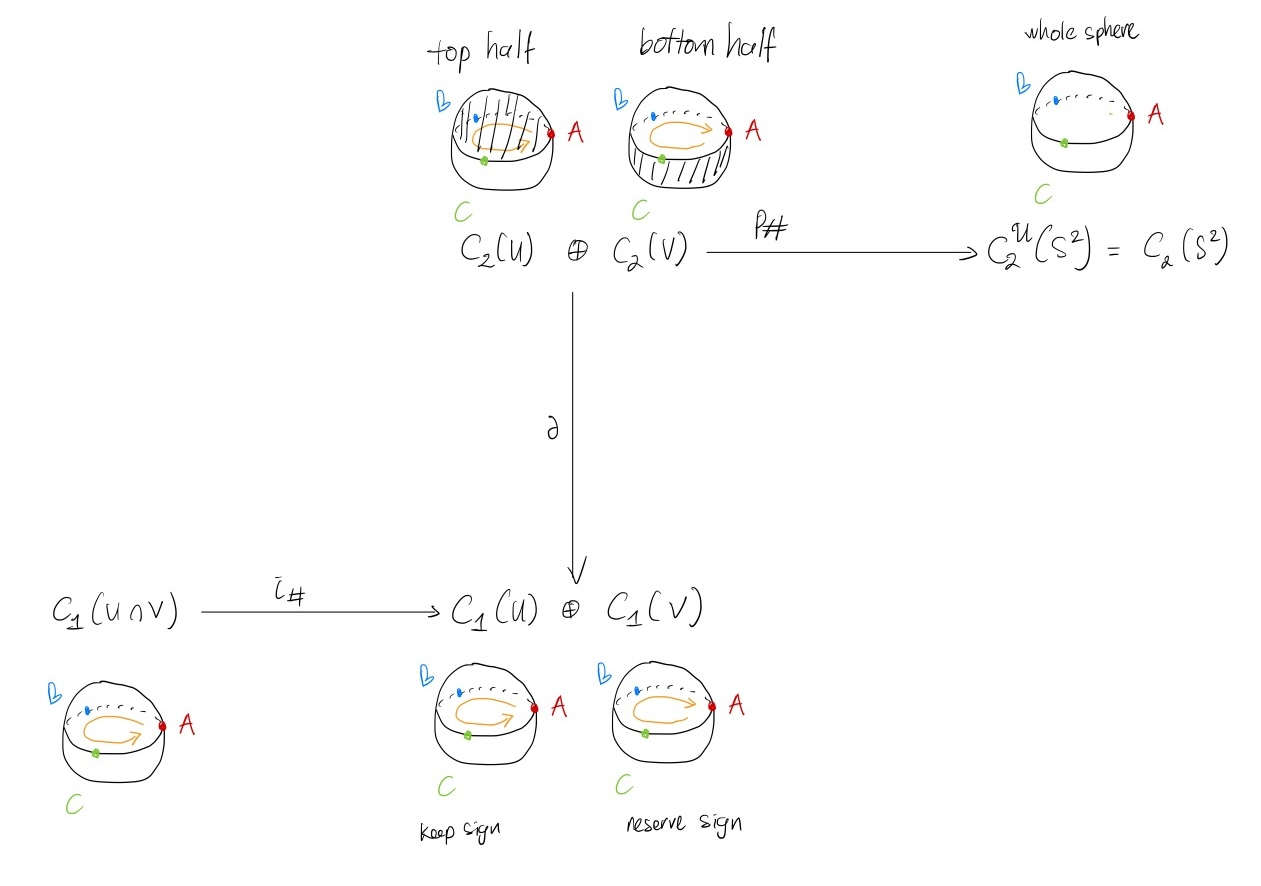
\includegraphics[width=0.7\textwidth]{3.2.jpg}
    \caption{A picture is worth a thousand words}
    \label{fig_3.2}
    \end{figure}
    
    Let $A, B, C$ be three distinct points on the equator. Let $a = AB + BC - AC \in C_1(U \cap V)$ be a singular $1$-chain on $S^2$ with $[a]$ being a generator of $H_1(U \cap V)$ ($xy$ denotes the path from $x$ to $y$). We will find $c \in C_2^\mathcal{U}(S^2)$ such that $\partial c = a$, then $[c]$ is a generator of $H_2(C_2^\mathcal{U}(S^2)) = H_2(S^2)$ similar to the previous part.
    
    We have $\partial b = (a, -a) \in C_1(U) \oplus C_1(V)$. Now, take $b = (\sigma_u, -\sigma_v^{AB} -\sigma_v^{BC} +\sigma_v^{AC}) \in C_2(U) \oplus C_2(V)$ where the mapping from vertices of $\Delta^2$ is as follows
    \begin{align*}
        \sigma_u &: 0 \mapsto A, 1 \mapsto B, 2 \mapsto C , N \in \im \sigma_u\\
        \sigma_v^{AB} &: 0 \mapsto S, 1 \mapsto A, 2 \mapsto B \\
        \sigma_v^{BC} &: 0 \mapsto S, 1 \mapsto B, 2 \mapsto C \\
        \sigma_v^{AC} &: 0 \mapsto S, 1 \mapsto A, 2 \mapsto C \\
    \end{align*}
    Then, $\partial \sigma_u = AB + BC - AC = a$, $\partial (-\sigma_v^{AB} - \sigma_v^{BC} + \sigma_v^{AC}) = -(SA + AB - SB) - (SB + BC - SC) + (SA + AC - SC) = -a$. The existence of $b$ can be proved by a sequence of maps: (1) projection of the half $2$-sphere the equatorial disk (2) affine map the equatorial disk to triangle $ABC$ (3) map triangle $ABC$ to $\Delta^2$. Finally, $c = \sigma_u -\sigma_v^{AB} -\sigma_v^{BC} + \sigma_v^{AC}$ with $[c]$ being a generator of $H_2(S^2)$


    
    Is there a homologous $2$-cycle consisting of just one simplex?
     Yes, consider the deformation $\gamma$ of image of $\sigma_u$ into $S^2$ such that $A, B, C \mapsto S$, then $\sigma = \gamma \circ \sigma_u$ ($\sigma$ covers the whole sphere and sends $0, 1, 2$ to $S$). We are left to prove that $- \sigma + c$ is a boundary where $c$ is a $2$-cycle and $[c]$ generates of $H_2(S^2)$ obtained from the previous process.

    \begin{figure}[h]
    \centering
    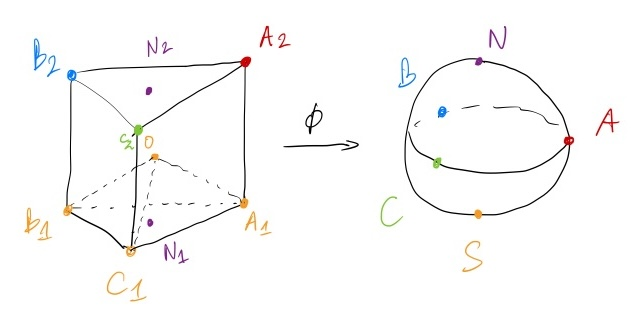
\includegraphics[width=0.7\textwidth]{3.3.jpg}
    \caption{A picture is worth a thousand words}
    \label{fig_3.3}
    \end{figure}

     Let a continuous map $\phi$ from a prism $\Delta^2 \times I$ to the closed ball as in figure \ref{fig_3.3} in such a way that
     \begin{itemize}
         \item $A_2 \mapsto A, B_2 \mapsto B, C_2 \mapsto B$
         \item $N_1, N_2 \mapsto N$
         \item $A_1, B_1, C_1, O \mapsto S$
     \end{itemize}
     where $N_1, N_2$ are centers of $A_1 B_1 C_1$ and $A_2 B_2 C_2$ respectively, $O$ is the center of the prism. Then, the boundary of $\phi$ generated by prism operators are exactly $B_2 C_2 A_2$, $C_1 A_1 A_2$, $C_1 C_2 A_2$, $B_1 C_1 C_2$, $B_1 B_2 C_2$, $B_1 B_2 A_2$, $B_1 A_1 A_2$ and $B_1 C_1 A_1$. The first $7$ $2$-simplices correspond to the $2$-cycle $c$ and the last $2$-simplex corresponds to $\sigma$. We claim that $\partial \phi = -\sigma + c$

    
\end{longproof}

\begin{problem}
    :
    \begin{enumerate}[label=(\roman*)]
        \item \label{4.1} Verify that the subdivision operators $\Sd_n: C_n(X) \to C_n(X)$ \textcolor{red}{(and the boundary operator)} together form a chain map
        \item \label{4.2} Recall the construction of an operator $T_n: C_n(X) \to C_{n+1}(X)$ such that
        $$
            \partial T_n + T_{n-1} \partial = 1 - \Sd_n
        $$
        We defined it by first specifying a chain $t_n \in C_{n+1}(\Delta^n)$ and then, for $\sigma: \Delta^n \to X$, defining $T_n(\sigma) = \sigma_\#(t_n)$. The chain $t_n$ was defined inductively by
        $$
            t_0 = 0, t_n = c_b(\iota_n - \Sd_n \iota_n - T_{n-1} \partial \iota_n)
        $$
        where $c_b$ is the cone operator with respect to barycentre and $\iota_n$ is the identity simplex in $S_n(\Delta^n)$. Draw pictures of the relevant singular simplices in $\Delta^1$ to verify that $\partial t_1 = \iota_1 - \Sd \iota_1$
        \item \label{4.3} Verify that the inclusion of the $\mathcal{U}$-small chains into all chains is not just an isomorphism in homology, but in fact that there is a chain homotopy inverse
    \end{enumerate}
\end{problem}

\begin{longproof}
    \ref{4.1}

    Without confusion, we will use $\sd_n: C_n(\Delta^\bullet) \to C_n(\Delta^\bullet)$ to denote the subdivision operator on space of simplices (Euclidean space), $\Sd_n: C_n(X) \to C_n(X)$ to denote the subdivision operator on an arbitrary topological space $X$ and defined by $\Sd_n \sigma_\# = \sigma_\# \sd_n$. That is equivalent to, $\Sd_n \sigma = \Sd_n \sigma_\# 1 = \sigma_\# \sd_n 1$ where $1: \Delta^n \to \Delta^n$ is the identity map. 
    
    We will first prove the naturality of $\sd_\bullet$, that is, $\partial \sd_n = \sd_{n-1} \partial$ using an inductive argument. Base case: let $\sigma: \Delta^1 \to \Delta^\bullet$,
    \begin{align*}
        \partial \sd_1 \sigma
        &= \partial c_{b(1)} sd_0 \partial \sigma \\
        &= \partial c_{b(1)} \partial \sigma \\
        &= \partial c_{b(1)} \partial \sigma \\
        &= (1 - b \epsilon) \partial \sigma \\
        &= \partial \sigma - b \epsilon \partial \sigma \\
        &= \partial \sigma - b \epsilon (\sigma(1) - \sigma(0)) &\text{($\sigma$ is $1$-dimensional, $\sigma(x)$ denotes $\Delta^0 \mapsto \sigma(x)$)}\\
        &= \partial \sigma - b 0 &\text{($\sigma(0), \sigma(1) \in S_0(\Delta^\bullet)$, definition of augmentation map)}\\
        &= \partial \sigma \\
        &= \partial \sd_0 \sigma
    \end{align*}
    
    where $c_{b(1)}$ denotes the cone operator with respect to the barycentre of $\Delta^1$. Now, given $\partial \sd_{n-1} = \sd_{n-2} \partial$, we will prove $\partial \sd_n = \sd_{n-1} \partial$ for $n > 1$. Let $\sigma: \Delta^n \to \Delta^\bullet$,
    \begin{align*}
        \partial \sd_n \sigma
        &= \partial c_{b(n)} \sd_{n-1} \partial \sigma &\text{(definition of $\sd_n$)}\\
        &= (1 - c_{b(n)} \partial) \sd_{n-1} \partial \sigma &\text{($\sd_{n-1} \partial \sigma$ is of $n-1 > 0$ dimensional)} \\
        &= \sd_{n-1} \partial \sigma - c_{b(n)} \partial \sd_{n-1} \partial \sigma \\
        &= \sd_{n-1} \partial \sigma - c_{b(n)} \sd_{n-1} \partial^2 \sigma &\text{(induction argument)}\\
        &= \sd_{n-1} \partial \sigma
    \end{align*}

    where $c_{b(n)}$ denotes the cone operator with respective to the barycentre of $\Delta^n$. Let $\sigma: \Delta^n \to X$, the naturality of $\Sd_n$ is a consequence of naturality of $\sd_n$ and $\sigma_\#$. 

\begin{center}
% https://tikzcd.yichuanshen.de/#N4Igdg9gJgpgziAXAbVABwnAlgFyxMJZARgBoAGAXVJADcBDAGwFcYkQBhAfTAAoAdfgBEYjHPQB6YAJQgAvqXSZc+QigAsFanSat23PoJFjJM+YpAZseAkQBMpAMzaGLNok49eADVkKl1qpEAKxOLrrunny+5gEqtihk6uFu+lzAYAC0xHI+fhZW8WrImsk0rnoe3BnZuTH+lso2xeSkxCmVnjU5AsKi4lL5cc1Ejm0dkdVZPUb9pn7aMFAA5vBEoABmAE4QALZIrSA4EEgOOqkegtjLu-RcggDEsSDbe6c0x0ia552CaPRbPBMZ6vfaIQ6fRBkH6RK5QHggnZg6GQsYw9hXLA3O6PRFvRBoyGhdGXfj-QFYYENUFfD4nRDEiqw-gAZXh3TkeLBZ1R5QiGNZ8MI1KRSAAbHSkAB2PkXEBw9LTTki-EQ+kSknyskAoGMLlIFH0mWav46yl6lVg41E2W-fjXW73fhPS3iyWIb5MgUOnHO+SUORAA
\begin{tikzcd}
                                                                     & C_n(\Delta^n) \arrow[rddd, "\sigma_\#"] \arrow[rrr, "\sd_n"] \arrow[ld, "\partial"] &                                                    &                                             & C_n(\Delta^n) \arrow[rddd, "\sigma_\#"] \arrow[ld, "\partial"] &                               \\
C_{n-1}(\Delta^n) \arrow[rrr, "\sd_{n-1}"] \arrow[rddd, "\sigma_\#"] &                                                                                     &                                                    & C_{n-1}(\Delta^n) \arrow[rddd, "\sigma_\#"] &                                                                &                               \\
                                                                     &                                                                                     &                                                    &                                             &                                                                &                               \\
                                                                     &                                                                                     & C_n(X) \arrow[ld, "\partial"] \arrow[rrr, "\Sd_n"] &                                             &                                                                & C_n(X) \arrow[ld, "\partial"] \\
                                                                     & C_{n-1}(X) \arrow[rrr, "\Sd_{n-1}"]                                                 &                                                    &                                             & C_{n-1}(X)                                                     &                              
\end{tikzcd}
\end{center}

    We have these commutative squares
    \begin{itemize}
        \item $\partial \sigma_\# = \sigma_\# \partial$
        \item $\partial \sd_n = \sd_{n-1} \partial$ (naturality of $\sd_n$)
        \item $\sigma_\# \sd_\bullet = \Sd_\bullet \sigma_\#$ (by definition of $\Sd_\bullet$)
    \end{itemize}
    
    Then,
    $$
        \partial \Sd_n \sigma_\# = \partial \sigma_\# \sd_n =  \sigma_\# \partial \sd_n = \sigma_\# \sd_{n-1} \partial = \Sd_{n-1} \sigma_\# \partial = \Sd_{n-1} \partial \sigma_\#
    $$

    Then, $\partial \Sd_n \sigma = \partial \Sd_n \sigma_\# 1 = \Sd_{n-1} \partial \sigma_\# 1 = \Sd_{n-1} \partial \sigma$ where $1: \Delta^n \to \Delta^n$ is the identity map. Hence, $\partial \Sd_n = \Sd_{n-1} \partial$

    \ref{4.2}

    As $T_0 = 0$
    $$
        t_1 = c_{b(1)} (\iota_1 - \Sd_1 \iota_1 - T_0 \partial \iota_1)
            = c_{b(1)} (\iota_1 - \Sd_1 \iota_1)
    $$
    
    Then, 
    \begin{align*}
        \partial t_1
        &= \partial c_{b(1)} (\iota_1 - \Sd_1 \iota_1) \\
        &= (1 - c_{b(1)} \partial) (\iota_1 - \Sd_1 \iota_1) &\text{($\iota_1 - \Sd_1 \iota_1 \in C_1(\Delta^\bullet)$)}\\
        &= \iota_1 - \Sd_1 \iota_1 - c_{b(1)} \partial (\iota_1 - \Sd_1 \iota_1)
    \end{align*}

    We verify $\partial \iota_1 - \partial \Sd_1 \iota_1  = 0$ by figure \ref{fig_4.1}

    \begin{figure}[h]
    \centering
    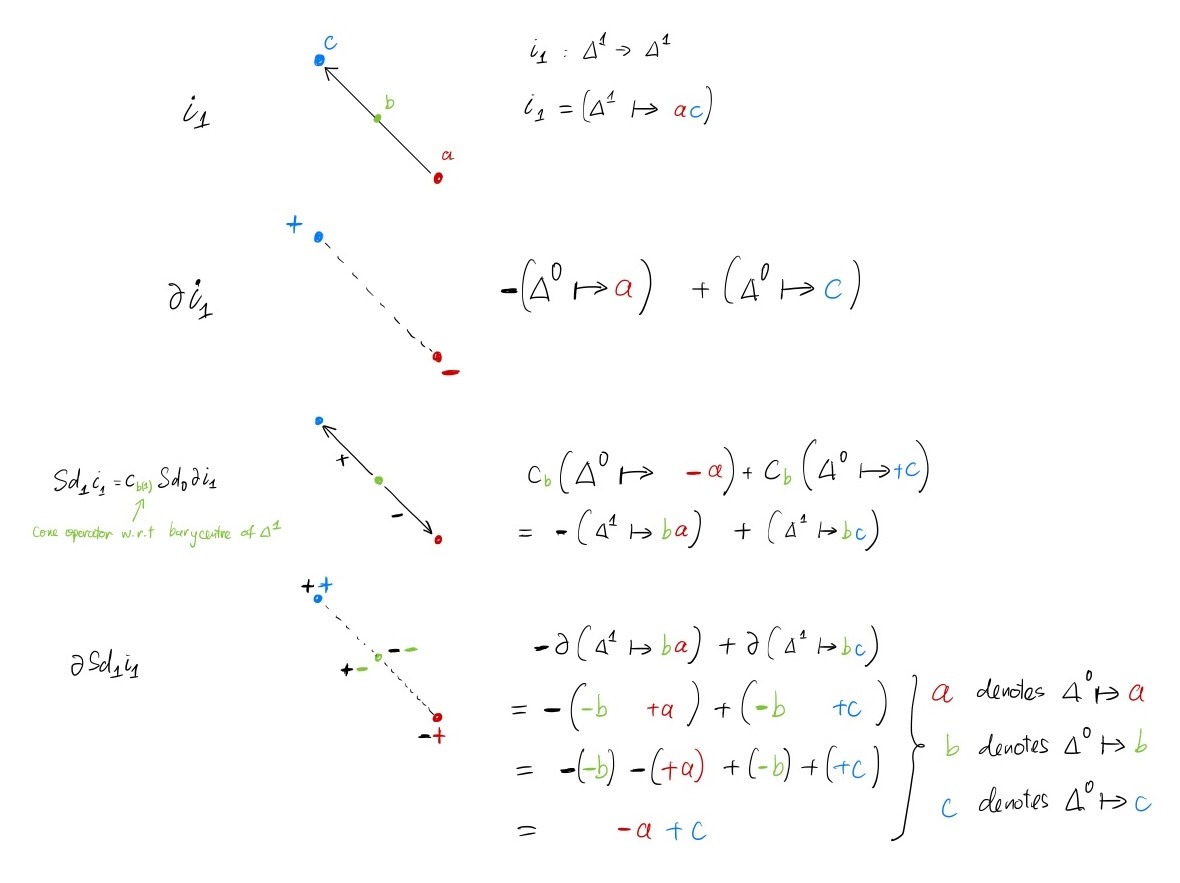
\includegraphics[width=0.7\textwidth]{4.1.jpg}
    \caption{A picture is worth a thousand words}
    \label{fig_4.1}
    \end{figure}
    
    \ref{4.3}

    Let $\mathcal{U}$ be an open cover of $X$. The locality principle asserts that the inclusion map $f: C^\mathcal{U}_n(X) \hookrightarrow C_n(X)$ is a chain homotopy equivalence, that is, there exists a map $g: C_n(X) \to C^\mathcal{U}_n(X)$ such that $g = gf: C^\mathcal{U}_n(X) \to C^\mathcal{U}_n(X)$ and $g = fg: C_n(X) \to C_n(X)$ are chain homotopic to $1$. We will construct such map $g$ satisfying chain homotopy equivalence.

    Let $T^{(k)} = (1 + \Sd + \Sd^2 + ... + \Sd^{k-1}) T$ be the chain homotopy from $\Sd^k$ to $1$, that is, $\partial T^{(k)} + T^{(k)} \partial = 1 - \Sd^k$. For each $\sigma \in S_n(X)$, there exists an integer $m$ such that $\Sd^k \sigma \in C^\mathcal{U}_n(X)$ for all $k \geq m$. Define $D: C_n(X) \to C_{n+1}(X)$ as a linear extension of $D: S_n(X) \to C_{n+1}(X)$ with $D \sigma = T^{(m)} \sigma$. Let $g: C_n(X) \to C^\mathcal{U}_n(X)$ be defined by $g = 1 - \partial D - D \partial$. We will verify the following (1) $g$ is a chain map (2) $\im g \subseteq C^\mathcal{U}_n(X)$. 

    Indeed, $g$ is a chain map because
    \begin{align*}
        \partial g &= \partial (1 - \partial D - D \partial) = \partial - \partial D \partial \\
        g \partial &= (1 - \partial D - D \partial) \partial = \partial - \partial D \partial \\
    \end{align*}

    Now, for each $\sigma \in S_n(X)$,
    \begin{align*}
        g \sigma
        &= (1 - \partial D - D \partial) \sigma \\
        &= \sigma - \partial T^{(m)} \sigma - D \partial \sigma \\
        &= \sigma - (1 - \Sd^m - T^{(m)} \partial) \sigma - D \partial \sigma \\
        &= \Sd^m \sigma + (T^{(m)} - D) \partial \sigma
    \end{align*}
    
    By the choice of $m$, $\Sd^m \sigma \in C^\mathcal{U}_n(X)$. Now, we write $\partial \sigma$ as a sum
    $$
        \partial \sigma = \sum_{i=1}^n (-1)^i d_i \sigma
    $$
    
    We have
    $$
        (T^{(m)} - D) d_i \sigma = (T^{(m)} - T^{(m_i)}) d_i \sigma
    $$

    where $m_i$ is the smallest integer such that $\Sd^{m_i} d_i \sigma \in C^\mathcal{U}_n(X)$. Since $d_i \sigma$ is a restriction of $\sigma$, $m_i \leq m$. Then
    $$
        (T^{(m)} - T^{(m_i)}) d_i \sigma = (\Sd^{m_i} + ... + \Sd^{m-1})T d_i \sigma
    $$

    $T d_i \sigma = (d_i \sigma)_\# t_{n-1}$ where $t_{n-1} \in C_n(\Delta^{n-1})$ and $d_i \sigma: \Delta^{n-1} \to X$. If we write $t_{n-1} = \sum a_k$ where each $a_k: \Delta^n \to \Delta^{n-1}$, then $(d_i \sigma)_\# t_{n-1} = \sum (d_i \sigma)_\# a_k = \sum \sigma d^i a_k$. We have $\im \sigma d^i a_k \subseteq \im \sigma$, then $\im T d_i \sigma \subseteq \im \sigma$. By the choice of $m_i$, each $\Sd^\bullet$ in $\Sd^{m_i} + ... + \Sd^{m-1}$ maps $\im \sigma$ into one of the open sets in $\mathcal{U}$. Therefore, $(\Sd^{m_i} + ... + \Sd^{m-1})T d_i \sigma \in C^\mathcal{U}_n(X)$
\end{longproof}

\begin{problem}
    Suppose that
    \begin{center}
        % https://tikzcd.yichuanshen.de/#N4Igdg9gJgpgziAXAbVABwnAlgFyxMJZAJgBoAGAXVJADcBDAGwFcYkQBhAfWDAGoAjAF8QQ0uky58hFAGYK1Ok1bsAgl0JiJ2PASIAWBTQYs2iEACENo8SAw7pRAKxGlp9t0237UvSgBsriYq5uq8ALTCNtq+MsgA7EHKZiDRdpK6cWQCisEp3LyCQgDkaT6ZRPI5xslqGqVa6Q5+yIbVbiGW9WUZjigu7Xke3Y3lfciBg7WhPGCRJT3NcYlT7uaLsUQCSWtdhVGjvS3bq51W+wuHS0TkO50bFSi3pymiijBQAObwRKAAZgAnCAAWyQtxAOAgSG2HRSAGsQDRGPQAEYwRgABSOMhAjBgfxwaUBIOhNEhSDIsPYWERuNR6Kx13MeIJRKBoMQMPJiESVPMAB1+Uw0AALei05FozHY9gswmNYkcync+R8kAAKwl9OlTNx+PltkVFLJUMQAA4artBWicOKkdrGZtmfq2STEKruYY1Qj7VLHY89ayFeykB7TQBOS2dQWfejA4H0AAEgoAxgRPlq-TLnUHDSHEF7uS4+WBmIxGL6GdnAwb-vnC6aBOChohS+XKzqnTXXRzAhDTbyWyA4aUO-6+t3g27edyLWqsKO6VndXKe0g59zI2r1YvJVWVy6pxyt9ym1H4buHdXV0foeDTzCW22K0v912b3m3QIw0g+0Od2unLKqazbTBqgECA20LELenLFqesiwQIwHQqqQ7WjAtqAfepp-mBMZxgmyb8mmYAZkIlBCEAA
        \begin{tikzcd}
        {} \arrow[r] & B_{n+1} \arrow[r, "j"] \arrow[d, "\beta"] & C_{n+1} \arrow[r, "k"] \arrow[d, "\gamma \cong"] & A_n \arrow[r, "i"] \arrow[d, "\alpha"] & B_n \arrow[r, "j"] \arrow[d, "\beta"] & C_n \arrow[r, "k"] \arrow[d, "\gamma \cong"] & A_{n-1} \arrow[r] \arrow[d] & {} \\
        {} \arrow[r] & B_{n+1}' \arrow[r, "j'"]                  & C_{n+1}' \arrow[r, "k'"]                         & A_n' \arrow[r, "i'"]                   & B_n' \arrow[r, "j'"]                  & C_n' \arrow[r, "k'"]                         & A_{n-1}' \arrow[r]          & {}
        \end{tikzcd}
    \end{center}

    is a "ladder": a map of long exact sequences. So both rows are exact and each square commutes. Suppose also that every third vertical map is an isomorphism, as indicated. Prove that these data determine a long exact sequence
    \begin{center}
        % https://tikzcd.yichuanshen.de/#N4Igdg9gJgpgziAXAbVABwnAlgFyxMJZARgBoAGAXVJADcBDAGwFcYkQAhAfWDAGpiAXwDkIQaXSZc+QigBMFanSat2AQS6Fxk7HgJEAzIpoMWbRCA1hhAAgA6diGhZwb3LRJAZdMogBZjZTN2d1FtLyk9WWQAVkDTVQsNXgBaITFPb2l9FAA2eJVzEAydbOjyAuCLMSUYKABzeCJQADMAJwgAWyQKkBwIJDIgxJAAa3s7evpOzvoAPWA0wQArURpGegAjGEYABUjfC0YYFpwSkHauwZp+pAVhooAKByY0AAt6UhsUrABKEHWWx2+x8ORAx1O50u3UQ91uiCMD3YDk2bXoAGNRjAcMAsMIvijsfRBADwUC9gcwRCzuFoUhEfCAkiLOMHFMZvNFkJVqSNtsKaDZOCTjTPHTEEz4XFmWBmIxGID+SCyuxqVCOjD8n0BohyIJKIIgA
        \begin{tikzcd}
        {} \arrow[r] & B_{n+1}' \arrow[r, "k \gamma^{-1}j'"] & A_n \arrow[r, "{(\alpha, -i)}"] & A_n' \oplus B_n \arrow[r, "{\bracket{i', \beta}}"] & B_n' \arrow[r, "k \gamma^{-1}j'"] & A_{n-1} \arrow[r] & {}
        \end{tikzcd}
    \end{center}
\end{problem}

Denotes the maps as follows
\begin{itemize}
    \item $(\alpha, -i): a \mapsto (\alpha a, -i a)$
    \item $\bracket{i', \beta}: (a', b) \mapsto i' a' + \beta b$
    \item $(k \gamma^{-1} j'): b' \mapsto k \gamma^{-1} j' b'$
\end{itemize}

We will prove the three equalities
\begin{itemize}
    \item $\im (\alpha, -i) = \ker \bracket{i', \beta}$
    \item $\im \bracket{i', \beta} = \ker (k \gamma^{-1} j')$
    \item $\im (k \gamma^{-1} j') = \ker (\alpha, -i)$
\end{itemize}

\begin{enumerate}

\item ($\im (\alpha, -i) \subseteq \ker \bracket{i', \beta}$) Let $a \in A_n$, as $i' \alpha = \beta i$
$$
    \bracket{i', \beta} (\alpha, -i) a = \bracket{i', \beta} (\alpha a, -i a) = i' \alpha a - \beta ia = 0
$$

\item ($\im \bracket{i', \beta} \subseteq \ker (k \gamma^{-1} j')$) Let $(a', b) \in A_n' \oplus B_n$, as $j'i' = 0$, $j' \beta = \gamma j$, $kj = 0$

$$
    (k \gamma^{-1} j')[i', \beta] (a', b) = (k \gamma^{-1} j')(i' a' + \beta b) = k \gamma^{-1} j' i' a' + k \gamma^{-1} j' \beta b = k \gamma^{-1} \gamma j b = k j b = 0
$$

\item ($\im (k \gamma^{-1} j') \subseteq \ker (\alpha, -i)$) Let $b' \in B_{n+1}'$, as $\alpha k = k' \gamma$, $k 'j' = 0$, and $ik = 0$

$$
    (\alpha, -i)(k \gamma^{-1} j')b' = \alpha k \gamma^{-1} j' b' - i k \gamma^{-1} j' b' = \alpha k \gamma^{-1} j' b' = k' \gamma \gamma^{-1} j' b' = k' j' b' = 0
$$

\item ($\im (\alpha, -i) \supseteq \ker \bracket{i', \beta}$) Let $(a', b) \in A_n' \oplus B_n$ such that $[i', \beta] (a', b) = i' a' + \beta b = 0$. Then
$$
    j' i' a' + j' \beta b = j' 0 = 0
$$

As $j' i' = 0$, $j' \beta = \gamma j$, then

$$
    \gamma j b = 0
$$

Multiply both sides by $\gamma^{-1}$,

$$
    j b = \gamma^{-1} 0 = 0
$$

Then $b \in \ker j = \im i$, there exists $a \in A_n$ such that $i a = b$. As $i' a' + \beta b = 0$, we have

$$
    i' a' + \beta i a = 0
$$

As $\beta i = i' \alpha$,
$$
    i' (a' + \alpha a) = i' a' + i' \alpha a = 0
$$

As $a' + \alpha a \in \ker i' = \im k'$, there exists $c' \in C_{n+1}'$ such that $k' c' = a' + \alpha a$. Now, $k \gamma^{-1} c' - a \in A_n$ and

\begin{align*}
    (\alpha, -i)(k \gamma^{-1} c' - a)
    &= (\alpha (k \gamma^{-1} c' - a), - i(k \gamma^{-1} c' - a)) \\
    &= (\alpha k \gamma^{-1} c' - \alpha a, - ik \gamma^{-1} c' + ia) \\
    &= (k' c' - \alpha a, ia) &\text{($\alpha k = k' \gamma, ik = 0$)} \\
    &= (\alpha', b) &\text{($k' c' = a' + \alpha a$, $ia = b$)}
\end{align*}

\item ($\im \bracket{i', \beta} \supseteq \ker (k \gamma^{-1} j')$)

Let $b' \in B_n'$ such that $k \gamma^{-1} j' b' = 0$. $\gamma^{-1} j' b' \in \ker k = \im j$, then there exists $b \in B_n$ such that $jb = \gamma^{-1} j' b'$. As $\gamma j = j' \beta$,

$$
    j' \beta b = \gamma j b = j'b'
$$

Then, $j'(b' - \beta b) = 0$. As $b' - \beta b \in \ker j' = \im i'$, there exists $a' \in A_n'$ such that $i' a' = b' - \beta b$. Now, $(a', b) \in A_n' \oplus B_n$ and

\begin{align*}
    [i', \beta] (a', b)
    &= i' a' + \beta b \\
    &= b' - \beta b + \beta b &\text{($i' a' = b' - \beta b$)}\\
    &= b'
\end{align*}

\item ($\im (k \gamma^{-1} j') \supseteq \ker (\alpha, -i)$)

Let $a \in A_n$ such that $(\alpha, -i) a = (\alpha a, -ia) = (0, 0)$. As $a \in \ker i = \im k$, there exists $c \in C_{n+1}$ such that $k c = a$. As $k' \gamma = \alpha k$

$$
    k' \gamma c = \alpha k c = \alpha a = 0
$$
Then, $\gamma c \in \ker k' = \im j'$, there exists $b' \in B_{n+1}'$ such that $j' b' = \gamma c$. Now, $b' \in B_{n+1}'$ and

\begin{align*}
    k \gamma^{-1} j' b'
    &= k c &\text{($j' b' = \gamma c$)} \\
    &= a &\text{($k c = a$)}
\end{align*}

\end{enumerate}




\end{document}
